\documentclass[slidestop,compress,mathserif,10pt]{beamer}

\mode<article> % 仅应用于article版本
{
  \usepackage{beamerbasearticle}
%  \usepackage{fullpage}
  \usepackage{hyperref}
}

%% 下面的包控制beamer的风格,可以根据自己的爱好修改
\usepackage{beamerthemesplit}   % 使用split风格
\usepackage{beamerthemeshadow}  % 使用shadow风格
%\usepackage[width=2cm,dark,tab]{beamerthemesidebar}
%\usepackage{beamerthemetree}
%\usetheme{Montpellier}
%\usecolortheme{lily}


%% 这些包是可能会用到的,不必修改
\usepackage{amsmath,amssymb}
\usepackage{graphicx}
%\usepackage{color}
%\usepackage{pgf,pgfarrows,pgfnodes,pgfautomata,pgfheaps}
%\usepackage{multimedia}

%\documentclass{beamer}
%\usepackage{beamerthemeshadow}
\usepackage{beamerthemesplit}
%\usetheme{shadow}
\usepackage{graphicx}
\usecolortheme{lily}
%\usepackage{amsmass}
\usepackage{amssymb,amsfonts,url}
\graphicspath{{Problems/}}

%\usepackage{CJK}
%\usepackage{pinyin}

%    \begin{figure}
%        \centering
%        \includegraphics[width=0.8\textwidth]{newGeneRep.eps}
%    \end{figure}

% \begin{figure}%
%   \begin{center}%
%     \begin{minipage}{0.70\textwidth}%
%      \includegraphics[width=1.0\textwidth]{comp25000.eps}%
%     \end{minipage}%
%     \begin{minipage}{0.30\textwidth}
%      \includegraphics[width=1.0\textwidth]{comparelabel.eps}%
%     \end{minipage}%
%   \end{center}
% \end{figure}

% \begin{table}
%   {\begin{tabular}{l|rrr}\hline
%       & \multicolumn{3}{c}{Actual number of DCJ operations}\\
%       \# genes &\# genes $\times 1$&\# genes $\times 2$&\# genes  $\times 3$ \\
% \hline
%      (a)~25,000 & 0.5\% ~~&  0.9\% ~~& 1.7\%~~\\
%       (b)~10,000 & 0.8\%~~ &  1.4\% ~~& 2.7\%~~\\
%      (c)~ 1,000 & 2.7\%~~ & 4.7\%~~ & 14.7\%~~\\ \hline
%     \end{tabular}} {}%
% \end{table}

% \begin{eqnarray}
% T(n) &=&  \sum\nolimits_{i=1}^n C_i \\
%      &=&  \# PUSH + \#POP \\
%      &<& 2\times \#PUSH \\
%      &<& 2n \\
% \end{eqnarray}

% \[ 
% \begin{matrix}
% \begin{pmatrix}
% C_{11} & C_{12} \\ 
% C_{21} & C_{22} 
% \end{pmatrix}
% =
% \begin{pmatrix}
% A_{11} & A_{12} \\ 
% A_{21} & A_{22}  
% \end{pmatrix}
% 
% \begin{pmatrix}
% B_{11} & B_{12} \\ 
% B_{21} & B_{22}  
%  
% \end{pmatrix}
%     
%    \end{matrix}
% \]
% 
% 
% \begin{eqnarray}
%  C_{11} &=& (A_{11}\times B_{11}) + (A_{12} \times B_{21}) \\
% C_{12} &=& (A_{11}\times B_{12}) + (A_{12} \times B_{22}) \\
% C_{21} &=& (A_{21}\times B_{11}) + (A_{22} \times B_{21}) \\
% C_{22} &=& (A_{21}\times B_{12}) + (A_{22} \times B_{22}) 
% \end{eqnarray}
% \begin{figure}%
%      \begin{minipage}{0.32\textwidth}%
%       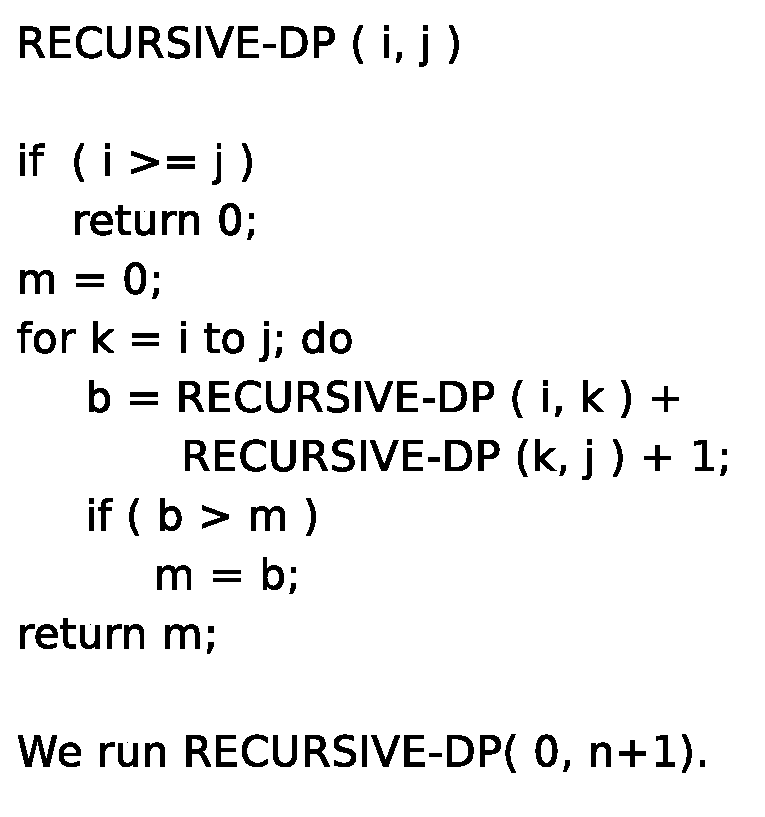
\includegraphics[width=1.0\textwidth]{L7-intervalschedulingdpalgo.eps}%
%      \end{minipage}%
%  \quad
%      \begin{minipage}{0.30\textwidth}
%       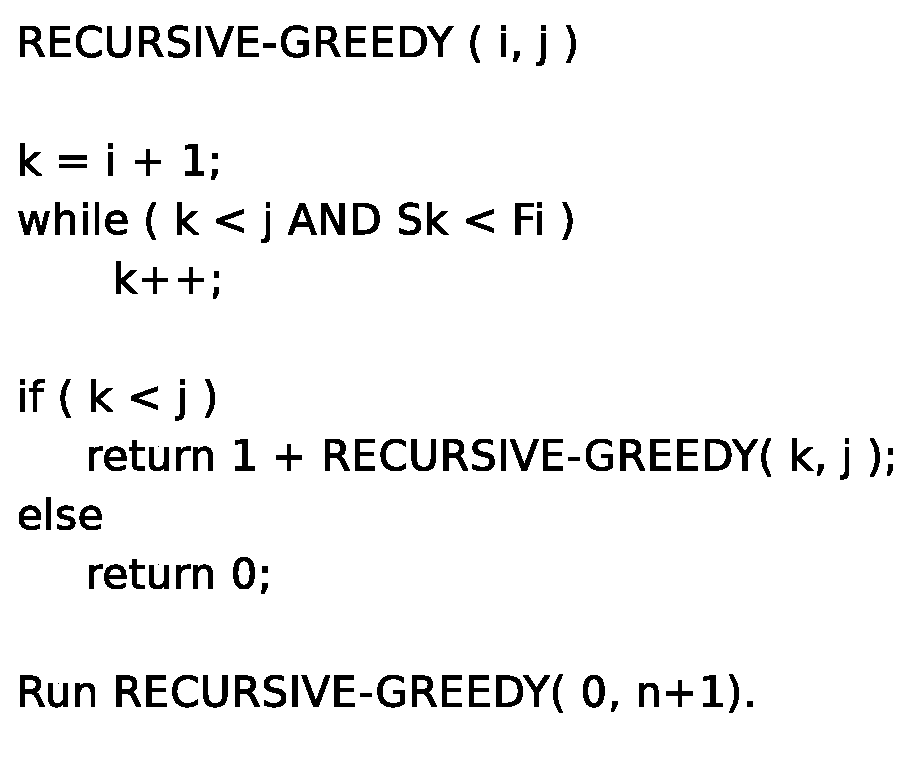
\includegraphics[width=1.0\textwidth]{L7-intervalschedulinggreedyalgo.eps}%
%      \end{minipage}%
%  \quad
%       \begin{minipage}{0.25\textwidth}
%       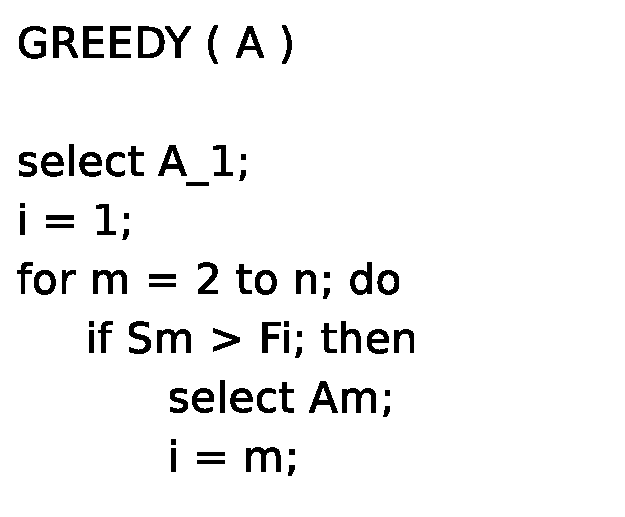
\includegraphics[width=1.0\textwidth]{L7-intervalschedulinggreedyalgo2.eps}%
%      \end{minipage}%
% 
%  \end{figure}

\title{CS612  Algorithm Design and Analysis }
\subtitle{ Lecture 18. {\sc ClosestString} and {\sc ClosestSubstring} problems: random sampling and random rounding
\footnote{The slides are made based on {\it On the closest string and substring problems} by M. Li, B. Ma, and L. Wang. } }
\author{Presented by Mingfu Shao \\
\ \\
{\small Institute of Computing Technology \\ 
Chinese Academy of Sciences, Beijing, China}}

\date{}

\begin{document}

%%
%% 填写作者,单位,日期,标题等文档信息
%%
%%%%%%%%%%%%%%%%%%%%%%%%%%%%%%%%%%%%%%%%%%%%%%%%%%%%%%%%%%%%%%%%%%%%%%%%%%%%%%%%%%%%%%%%%%%%%

\frame{\titlepage}

\frame[allowframebreaks]{
\frametitle{Outline}
\begin{itemize}
\item Problem statements; 
\item {\sc ClosestString } problem: random rounding technique; 
\item {\sc ClosestSubstring } problem: random sampling technique; 
\end{itemize}
}

\section{Problem Formulation}
\frame[allowframebreaks]
{
\frametitle{Problem Statement}
\begin{block}{\sc Closest String}
	Given a set $\mathcal{S} = \{s_1, s_2, \cdots, s_n\}$ of strings each length $m$, find a center string $s$ of length $m$ minimizing $d$
	such that for every string $s_i \in \mathcal{S}$, $d(s, s_i) \le d$. Here $d(s, s_i)$ is the Hamming distance between $s$ and $s_i$.
\end{block}

\begin{block}{\sc Closest Substring}
	Given a set $\mathcal{S} = \{s_1, s_2, \cdots, s_n\}$ of strings each length $m$ and an integer $L$, find a center string $s$ of length $L$
	minimizing $d$ such that for every string $s_i \in \mathcal{S}$ there is a length $L$ substring $t_i$ of $s_i$ with $d(s, t_i) \le d$.
\end{block}
}

\frame
{
\frametitle{Example of \sc Closest String}
Given 4 strings $s_1, s_2, s_3, s_4$,
\begin{figure}
	\begin{center}
		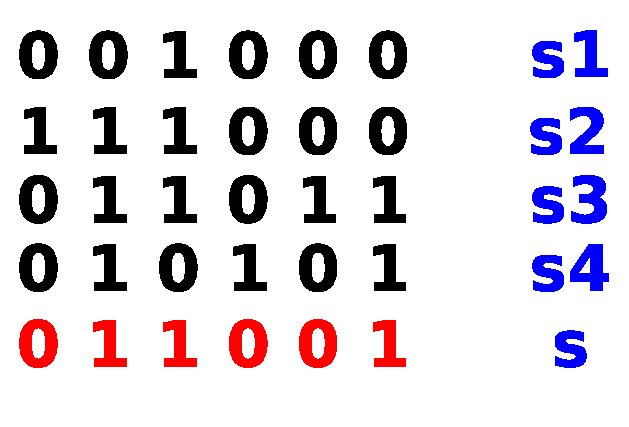
\includegraphics[width=0.5\textwidth]{cs.eps}
	\end{center}
\end{figure}
Optimal center string $s=011000$
\begin{eqnarray*}
	d=\max_{i=1}^4 d(s_i, s) = \max\{2,2,1,2\} = 2
\end{eqnarray*}
}

\frame
{
\frametitle{Example of \sc Closest Substring}
Given 4 strings $s_1, s_2, s_3, s_4$, $L=4$,
\begin{figure}
	\begin{center}
		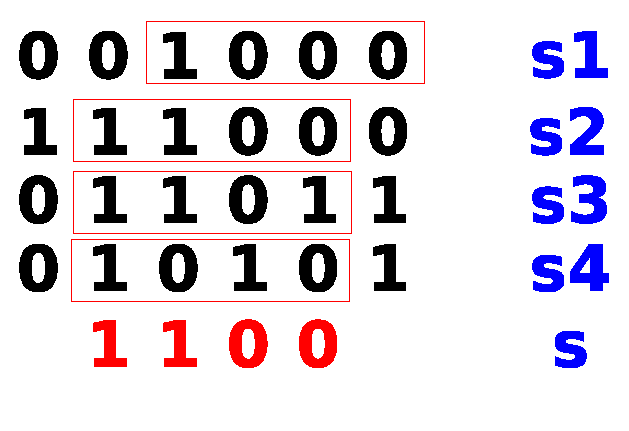
\includegraphics[width=0.5\textwidth]{css.eps}
	\end{center}
\end{figure}
Optimal center string $s=1100$,
\begin{eqnarray*}
	d=\max_{i=1}^4 d(t_i, s) = \max\{1,0,1,2\} = 2
\end{eqnarray*}
}
\section{Algorithm for Closest String Problem}
\frame
{
\frametitle{Basic Idea}

\begin{itemize} 

\item Applying ``LP+RR'' technique on all columns doesn't work due to the large size of the variables.  

\item 

In polynomial time, we can enumerate all ${n \choose r}$ strings for any fixed $r$. We can prove that, on positions that $r$ strings all agree, denote as $Q$, it is a good approximate solution; more speficially,  we can also prove that, $|Q| \ge m - r\cdot d_{opt}$.

\item 
On the other positions, we use LP + Random rounding technique to obtain an approximate solution.

\end{itemize}
%We want to employ LP-relaxation to solve the problem, but we meet difficulty that we do not know the relationship between $m$ and $d_{opt}$.

%In order for that, we use LP-relaxation only to a fraction of the $m$ positions, denote as $P$. We can prove 2 things: first $|P| < r\cdot d_{opt}$,
%second, on the left positions, we can enumerate all $r$-element subset to obtain a ``good enough'' partial solution in polynomial time.
}


\frame[allowframebreaks]
{
\frametitle{Algorithm}
{\bf Input : } $s_1, s_2, \cdots, s_n \in \Sigma^m$, an integer $r \ge 2$ and a small number $\epsilon > 0$.\\
{\bf Output : } a center string $s\in \Sigma^m$\\ 
{\bf Algorithm : }
\begin{enumerate}
	\item {\bf for} each $r$-element subset $\{s_{i_1}, s_{i_2}, \cdots, s_{i_r}\}$ of the $n$ input strings {\bf do}
		\begin{enumerate}
			\item let $Q=\{j|s_{i_1}[j] = s_{i_2}[j] = \cdots = s_{i_r}[j]\}$, $P=\{1,2,\cdots, m\} - Q$
			\item solve the following optimization problem
				\begin{eqnarray*}
					&&\min d\\
					s.t. && d(s_i|_P, y) + d(s_i|_Q, s_{i_1}|_Q) \le d, i=1,2,\cdots,n
				\end{eqnarray*}
				Random rounding the fractional solution $\bar{y}$ to get a approximation solution $y$. 
				Use derandomization technique to make this step deterministic rather than random.
			\item let $s'|_Q = s_{i_1}|_Q, s'|_P = y$. Calculate the radius of the solution with $s'$ as the center string.
		\end{enumerate}
	\item {\bf for } $i = 1,2,\cdots,n$ {\bf do}
		\begin{enumerate}
			\item calculate the radius of the solution with $s_i$ as the center string.
		\end{enumerate}
	\item output the best solution of the above two steps.
\end{enumerate}
}

\frame[allowframebreaks]
{
\frametitle{Example of \sc Closest String}
Suppose $r=2$. In step 1, we should enumerate all ${4 \choose 2} = 6$ cases. In each cases, we select $2$ lines, calculate $P$ and $Q$.
\begin{figure}
	\begin{center}
		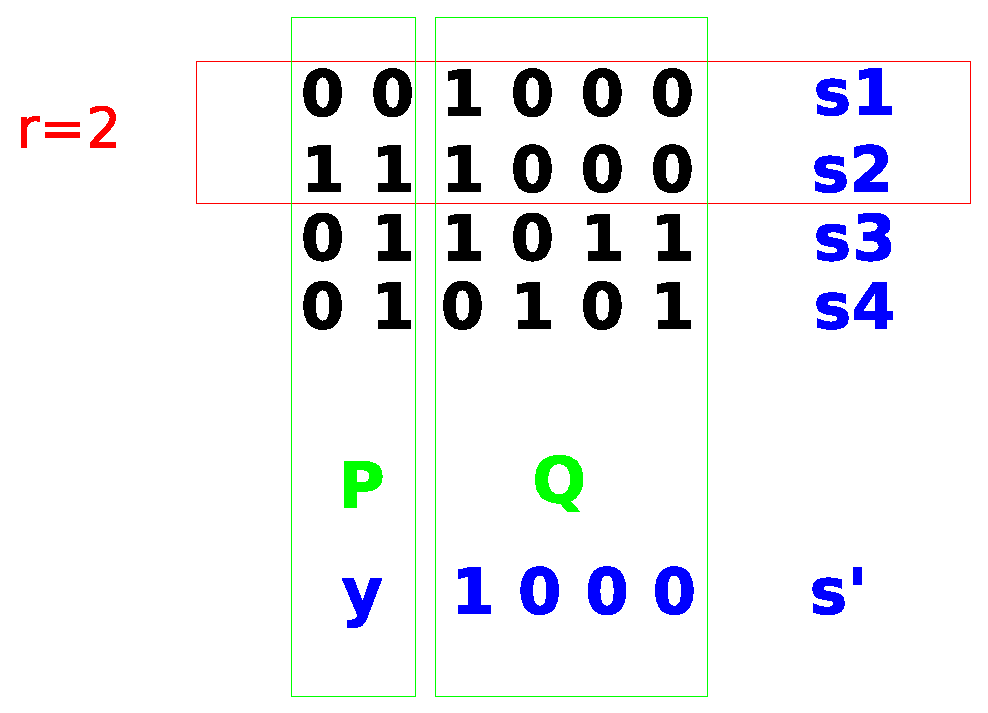
\includegraphics[width=0.6\textwidth]{csalgo1.eps}
	\end{center}
\end{figure}

In step 2, we fix $s'|_Q = 1000$, solve the following optimization problem :
\begin{eqnarray*}
	&& \min  d\\
	s.t. && y_{10} + y_{11} = 1\\
	 && y_{20} + y_{21} = 1\\
	 && y_{11} + y_{21} + 0 \le d \\
	 && y_{10} + y_{20} + 0 \le d \\
	 && y_{11} + y_{20} + 2 \le d \\
	 && y_{11} + y_{20} + 2 \le d \\
\end{eqnarray*}

Solve this linear programming, and random rounding the fractional solution to integer solution :
$$y_{10} = y_{21} = 1, y_{11} = y_{20} = 0$$
So, $$s'|_P = 01, s' = 011000$$
$$d=\max_{i=1}^4 d(s_i, s') = \max\{1,1,2,3\} = 3$$
Try all ${4 \choose 2} = 6$ cases, obtain the minimum, denote as $d_0$. Then we finish step 1.

In step 2, we calculate the radius when $s_i$ is the center string.
\begin{eqnarray*}
	d_1 & = & \max_{i=1}^4 d(s_1, s_i)\\
	d_2 & = & \max_{i=1}^4 d(s_2, s_i)\\
	d_3 & = & \max_{i=1}^4 d(s_3, s_i)\\
	d_4 & = & \max_{i=1}^4 d(s_4, s_i)
\end{eqnarray*}
Calculate the minimal radius in both step 1 and step 2.
$$d = \min\{d_0, d_1, d_2, d_3, d_4\}$$
}

\frame[allowframebreaks]
{
\frametitle{Analysis}
\begin{block}{Theorem}
	The above algorithm is a PTAS for {\sc Closest String} problem.
\end{block}

\begin{proof}
	Obviously, the time complexity of the algorithm is $O\left( (nm)^r n^{O(\log|\Sigma|\cdot r^2 / \epsilon^2)}\right)$, 
	which is polynomial in terms of $n$,$m$.\\

	The proof of approximation guarantee is organized as 3 lemmas as follows :\\
	Lemma 1 proves $s'|_Q$ is a good approximation to $s$ with approximation rate $1+\frac{1}{2r-1}$.\\
	Lemma 2 proves $|P| < r\cdot d_{opt}$.\\
	Based on the above 2 lemmas, 
	Lemma 3 proves step 1.2 obtains a approximate solution with rate $(1 + \frac{1}{2r-1} + \epsilon)$.

\end{proof}

\begin{block}{Lemma 1}
	If $\max_{i \le i,j \le n} d(s_i, s_j) > (1 + \frac{1}{2r-1})d_{opt}$,
	then there {\bf exists} $r$ indices $1 \le i_1, i_2, \cdots, i_r \le n$
	such that for any $1\le l \le n$,
	$$d(s_l|_Q, s_{i_1}|_Q) - d(s_l|_Q, s|_Q) \le \frac{1}{2r-1} d_{opt}$$
	where $Q$ is the set of positions that $s_{i_1}, s_{i_2}, \cdots, s_{i_r}$ all agree.
\end{block}

\begin{itemize}
	\item if $\max_{i \le i,j \le n} d(s_i, s_j) \le (1 + \frac{1}{2r-1})d_{opt}$, then any $s_i$ will be a good center string.
		(Recall the step 2 of the algorithm)
\end{itemize}

\begin{block}{Lemma 2}
	Let $P=\{1,2,\cdots, m\} - Q$, then $|P| \le r\cdot d_{opt}$ and $|Q| \ge m - r\cdot d_{opt}$.
\end{block}

\begin{proof}
	Let $q \in P$, then there exists some $s_{i_j}$ such that $s_{i_j}[q] \not = s[q]$. Since $d(s_{i_j}, s) \le d_{opt}$,
	each $s_{i_j}$ contributes at most $d_{opt}$ positions for $P$. Thus $|P| \le r\cdot d_{opt}$.
\end{proof}

\begin{itemize}
	\item this lemma gives the lower bound of $d_{opt}$, $d_{opt} \ge \frac{|P|}{r}$, which is essential for the analysis of LP + random rounding!
\end{itemize}


\begin{block}{Lemma 3}
	Given a string $s'$ and a position set $Q$ and $P$, $|P| < r\cdot d_{opt}$, such that for any $i=1,2,\cdots, n$,
	$$d(s_i|_Q,s'|_Q) - d(s_i|_Q, s|_Q) \le \rho \cdot d_{opt},$$
	then step 1.2 gives a solution with approximate rate $(1+\rho + \epsilon)$ in polynomial time for any fixed $\epsilon \ge 0$.
\end{block}

Before the proof, we can see that the conditions of this lemma are all satisfied by lemma 2, where $\rho = \frac{1}{2r-1}$.

{\bf Proof}

	Recall the optimization problem in step 1.2
	\begin{eqnarray*}
		&&\min d\\
		s.t. && d(s_i|_P, y) + d(s_i|_Q, s'|_Q) \le d, i=1,2,\cdots,n
	\end{eqnarray*}
	First, we show that $y=s|_P$ is a solution with cost $d \le (1+\rho)d_{opt}$. In fact, for $ i=1,2,\cdots,n$
	\begin{eqnarray*}
		& & d(s_i|_P, s|_P) + d(s_i|_Q, s'|_Q)\\ 
		& \le & d(s_i|_P, s|_P) + d(s_i|_Q, s|_Q) + \rho \cdot d_{opt} \\
		& \le & (1+\rho)d_{opt}
	\end{eqnarray*}
	
	Second, rewirte the optimization problem to an ILP problem. In order for this, 
	define 0-1 variables $y_{j,a}$, $1\le j \le |P|$, $a\in \Sigma$, $y_{j,a}=1$ means $y[j]=a$;
	define $\chi(s_i[j],a) = 0$ if $s_i[j]=a$ and $1$ if $s_i[j]\not=a$.
	Then the above optimization problem can be formulated as follows
	\begin{eqnarray*}
		&& \min d\\
		s.t. &&
		\begin{cases}
		\sum_{a\in \Sigma} y_{j,a} = 1, 1\le j \le|P|\\
		\sum_{1\le j\le |P|} \sum_{a\in \Sigma} \chi(s_i[j], a) y_{j,a} + d(s_i|_Q, s'|_Q) \le d, 1\le i\le n
		\end{cases}
	\end{eqnarray*}
	Solve it by LP to get a fractional solution $\bar{y}$ with cost $\bar{d}$.\\
	Random rounding $\bar{y}$ to $y'$ by  independently set $y'_{j,a} = 1$ and $y'_{j,b}=0, b\in \Sigma - \{a\}$ with probability $\bar{y_{j,a}}$.\\
	So $d(s_i|_P, y') = \sum_{i=1}^{|P|} \sum_{a\in\Sigma}  \chi(s_i[j], a) y_{j,a}$, which is the sum of $|P|$ independent random variables.\\
	\begin{eqnarray*}
		E(d(s_i|_P)) & = & \sum_{1\le j\le |P|} \sum_{a\in \Sigma} \chi(s_i[j], a) \bar{y_{j,a}} \\
	& \le &\bar{d} -  d(s_i|_Q, s'|_Q) \\
	& \le & (1+\rho)\cdot d_{opt} - d(s_i|_Q, s'|_Q) 
	\end{eqnarray*}
	Employ Chernoff Bound
	$$\Pr(X > \mu + \epsilon n) \le \exp(-\frac{1}{3}n\epsilon^2)$$
	we have
	\begin{eqnarray*}
		\Pr(d(s_i|_P, y') > (1+\rho)d_{opt} - d(s_i|_Q, s'|_Q) + \epsilon'|P|) \le  \exp(-\frac{1}{3}\epsilon'^2|P|)
	\end{eqnarray*}
	Let $s'|_P = y'$ and consider all $n$ strings, we claim
	\begin{eqnarray*}
		\Pr(d(s_i, s') < (1+\rho)d_{opt} + \epsilon'|P| \textrm{ for all i}) \ge  1 - n \exp(-\frac{1}{3}\epsilon'^2|P|)
	\end{eqnarray*}
	Use standard derandomization methods, we can obtain a deterministic $s'$ that satisfies
	$$d(s_i, s') < (1+\rho)d_{opt} + \epsilon'|P|, \quad 1\le i \le n$$
	Recall that $|P| < r\cdot d_{opt}$, let $\epsilon' = \frac{\epsilon}{r}$, we have
	$$d(s_i, s') < (1+\rho + \epsilon)d_{opt}, \quad 1 \le i \le n$$
	Then we finish the proof.
}

\section{Algorithm for {\sc Closest Substring} problem}

\frame
{
\frametitle{Basic Idea}

\begin{itemize} 
 \item 

We want to follow the algorithm of {\sc Closest String} algorithm. However, there is an obstacle: we do not know how to construct an optimization problem, for the reason that we do not konw the optimal substring in each string. Thus, the choice of a ``good'' substring from every string $s_i$
is the only obstacle on the way to the solution.\\

\item There is a ``dead cycle'': 
\begin{enumerate} 
 \item Suppose we know the center substring $s^*$, the optimal $t_i$ can be easily determined through comparison within a sliding window. 
 \item On the other hand, suppose we know all the optimal substrings $t_i$, $s^*$ can also be approximated using the {\sc ClosestString} algo. 
\end{enumerate}

\item How to break this cycle? Random sampling!

\item Speficically, we first randomly sample $O(log m n )$ positions $R$. By trying all length $|R|$ strings, we can assume we know $s|_R$.  The performance of these positions can be used to estimate the performance on all positions, i.e., for each $i\le i \le n$, we find the substring $t'_i$ from $s_i$
such that $f(t'_i) = d(s|_R, t'_i|_R)\cdot \frac{|P|}{|R|} + d(t_{i_1}|_Q, t'_i|_Q)$ is minimized. 
We use $t'_i, 1\le i \le n$ to construct the optimization problem.

 \end{itemize}
}

\frame[allowframebreaks]
{
\frametitle{Algorithm for {\sc Closest Substring} problem}
{\bf Input : } $s_1, s_2, \cdots, s_n \in \Sigma^m$, an integer $1 \le L \le m$, an integer $r \ge 2$ and a small number $\epsilon > 0$.\\
{\bf Ouput : } center string $s$\\
{\bf Algorithm : }\\
\begin{enumerate}
	\item {\bf for} each $r$-element subset $\{t_{i_1}, t_{i_2}, \cdots, t_{i_r}\}$, where $t_{i_j}$ is a substring of length $L$ from $s_{i_j}$ {\bf do}
		\begin{enumerate}
			\item let $Q=\{j|t_{i_1}[j] = t_{i_2}[j] = \cdots = t_{i_r}[j]\}$, $P=\{1,2,\cdots, m\} - Q$
			\item randomly select $\frac{4}{\epsilon^2}\log(mn)$ positions from $P$, denote as $R$
			\item {\bf for} every string $x$ of length $|R|$ {\bf do}
				\begin{enumerate}
					\item for $1 \le i \le n$, let $t'_i$ be a length $L$ substring of $s_i$ minimizing 
								$f(t'_i) = d(x, t'_i|_R)\cdot \frac{|P|}{|R|} + d(t_{i_1}|_Q, t'_i|_Q)$.
					\item solve the optimization problem
						\begin{eqnarray*}
							&& \min d\\
							s.t. && d(t'_i|_P,y) + d(t'_i|_Q, t_{i-1}|_Q) \le d, 1 \le i \le n
						\end{eqnarray*}
						Random rounding the fractional solution $\bar{y}$ to get a approximation solution $y$. 
						Use derandomization technique to make this step deterministic rather than random.
					\item Let $s'|_Q = t_{i_1}|_Q$ and $s'|_P = y$. Let $c = \max_{i=1}^n d(s', t'_i)$.
				\end{enumerate}
		\end{enumerate}
	\item {\bf for} every length $L$ substring $s'$ of $s_1$ {\bf do}
		\begin{enumerate}
			\item Let $c = \max_{i=1}^n \min_{t_i} d(s', ti)$.
		\end{enumerate}

	\item output the $s'$ with minimum $c$ in step 1.3.3 and step 2.1.
\end{enumerate}
}

\frame[allowframebreaks]
{
\frametitle{Example of \sc Closest Subtring}
Suppose $r=2$. In step 1, we should enumerate all ${4 \choose 2} \times 3 \times 3 = 54$ cases. 
In each cases, we select $2$ substring of length $4$ , calculate $P$ and $Q$.

We fix $s'|_Q = 00$.\\
Randomly select $|R| = O(\log(mn))$ positions, say, $|R| = 1$.
Then enumerate all length $|R|$ strings, say, $s'|_R = 0$.\\

\begin{figure}
	\begin{center}
		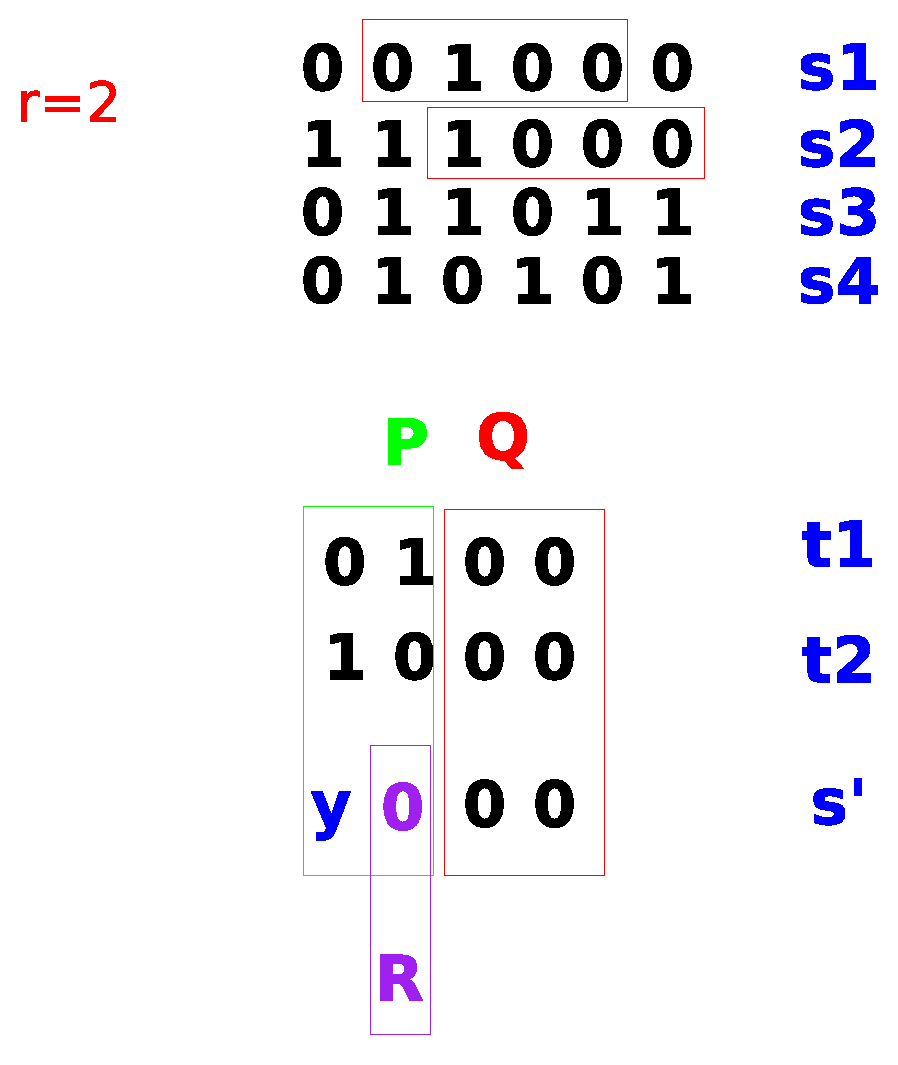
\includegraphics[width=0.5\textwidth]{cssalgo1.eps}
	\end{center}
\end{figure}

Now, for each $s_i$, find out the $t'_i$ minimizing $f(u) = d(u|_R, s'|_R) \times 2 + d(u|_Q, s'|_Q)$.
\begin{figure}
	\begin{center}
		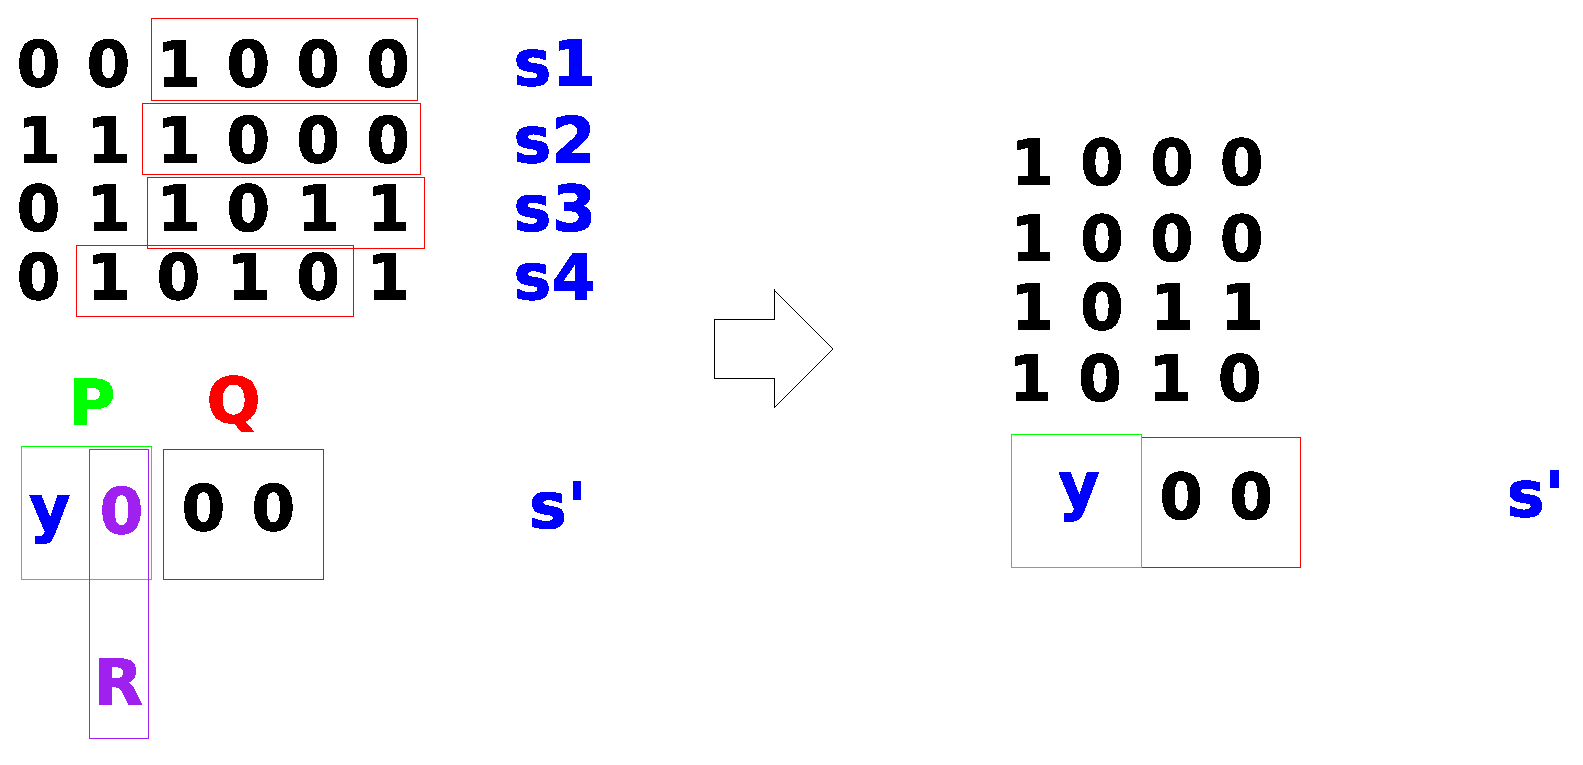
\includegraphics[width=0.6\textwidth]{cssalgo2.eps}
	\end{center}
\end{figure}


Solve the following optimization problem :

\begin{eqnarray*}
	&& \min  d\\
	s.t. && y_{10} + y_{11} = 1\\
	 && y_{20} + y_{21} = 1\\
	 && y_{10} + y_{21} + 0 \le d \\
	 && y_{10} + y_{21}  + 0 \le d \\
	 && y_{10} + y_{21} + 2 \le d \\
	 && y_{10} + y_{21} + 1 \le d \\
\end{eqnarray*}

Solve this linear programming, and random rounding the fractional solution to integer solution :
$$y_{10} = y_{21} = 0 , y_{11} = y_{20} = 1 $$
So, $$s' = 1000$$
$$d=\max_{i=1}^4 d(t_i, s') = \max\{0,0,2,1\} = 2$$
Try all $54$ cases, obtain the minimum, denote as $d_0$. Then we finish step 1.

In step 2, we calculate the radius when $t_i$ is the center string where $t_i$ is a length $L$ substring of $s_i$.
denote the minimun $d_1$.
Calculate the minimal radius in both step 1 and step 2.
$$d = \min\{d_0, d_1\}$$
}


\frame[allowframebreaks]
{
\frametitle{Analysis}
\begin{block}{Theorem}
	The above algorithm is a PTAS for {\sc Closest Substring} problem.
\end{block}

\begin{proof}
	The time complexity of the algorithm is $O\left( (n^m)^{O(\log|\Sigma|/ \delta^4)}\right)$, 
	which is polynomial in terms of $n$,$m$.\\

	The proof of approximation guarantee is organized as 3 lemmas as follows :\\
	Lemma 1 proves $s'|_Q$ is a good approximation to $s$ with approximation rate $1+\frac{1}{2r-1}$.\\
	Define $s^*|_P = s|_P$ and $s^*|_Q = t_{i_1}|_Q$, lemma 2 proves $d(s^*, t'_i) \le d(s^*, t_i) + 2\epsilon |P|$ for all $1\le i \le n$.\\
	Based on the above 2 lemmas, 
	Lemma 3 proves the algorithm obtains a approximate solution with rate $(1 + \frac{1}{2r-1} + 3\epsilon r)$.
\end{proof}

\begin{block}{Lemma 1}
	There exists $t_{i_1}, t_{i_2}, \cdots, t_{i_r}$ chosen in step 1, such that for any $1\le l \le n$
	$$d(t_l|_Q, t_{i_1}|_Q) - d(s_l|_Q,s|_Q) \le \frac{1}{2r-1}\cdot d_{opt}$$
\end{block}

\begin{proof}
	The fact follow from Lemma 1 of {\sc Closest String} directly.
\end{proof}


\begin{block}{Lemma 2}
	Define $s^*|_P = s|_P$ and $s^*|_Q = t_{i_1}|_Q$. Then we have, with high probability
  $$d(s^*, t'_i) \le d(s^*, t_i) + 2\epsilon |P|$$ for all $1\le i \le n$.
\end{block}

\begin{proof}
\end{proof}

\begin{itemize}
	\item The randomness comes from the randomly selected $|R|$. Use standard method, we can derandomize it to make this deterministic.
\end{itemize}

\begin{block}{Lemma 3}
	step 1.3.3 gives an approximation solution $s'$ with approximation rate $(1 + \frac{1}{2r-1} + 3\epsilon r)$.
\end{block}

{\bf Proof.}\\
	Recall the optimization problem in step 1.2
	\begin{eqnarray*}
		&&\min d\\
		s.t. && d(t'_i|_P, y) + d(t'_i|_Q, s'|_Q) \le d, i=1,2,\cdots,n
	\end{eqnarray*}
	$y=s|_P$ is a feasible solution. Now we calculate its radius when $s^*$ is the center string. Recall that $s^*|_P = s|_P$ and $s^*|_Q = t_{i_1}|_Q$.\\
	According to Lemma 2 and Lemma 1
	\begin{eqnarray*}
		d(s^*, t'_i) & \le & d(s^*, t_i) + 2\epsilon|P| \\
		& \le & d(s|_P, t_i|_P) + d(t_{i_1}|_Q, t_i|_Q) + 2\epsilon|P| \\
		& \le & d(s|_P, t_i|_P) + d(s|_Q, t_i|Q) + 2\epsilon|P| + \frac{1}{2r-1}d_{opt}\\
		& \le & (1 + \frac{1}{2r-1})d_{opt} + 2\epsilon|P|)
	\end{eqnarray*}
	
	In a short word, $y=s|_P$ is a solution of the optimization problem with cost at most $ (1 + \frac{1}{2r-1})d_{opt} + 2\epsilon|P|)$.

	Next, as we do in the {\sc Closest String} problem, we rewirte the optimization problem to an ILP and solve it and random rounding the 
	fractional solution $\bar{y}$ to $y$. Define $s'|_Q = t_{i_1}|_Q$ and $s'|_P = y$.\\
	$$E(d(s', t'_i)) \le \bar{d} \le  (1 + \frac{1}{2r-1} + 2\epsilon|P|) d_{opt}$$
	So, chernoff bound ensures that, with high probability, 
	\begin{eqnarray*}
		&& d(s', t'_i)\\
		& \le & (1 + \frac{1}{2r-1})d_{opt} + 2\epsilon|P| + \epsilon|P|\\
		& \le & (1 + \frac{1}{2r-1})d_{opt} + 3\epsilon|P|\\
		& \le & (1 + \frac{1}{2r-1} + 3\epsilon r) d_{opt}
	\end{eqnarray*}
 
	After derandomization, we can obtain an approximation solution $s'$ with rate $ (1 + \frac{1}{2r-1} + 3\epsilon r) d_{opt}$.

}

\end{document}
